%%%%%%%%%%%%%%%%%%%%%%%%%%%%%%%%%%%%%%%%%%%%%%%%%%%%%%%%%%%%%%%%%
% Contents: Main Input File - Diplomarbeit, FH Regensburg       %
%                          11.03.2003                           %
%---------------------------------------------------------------%
%                       Diplomarbeit.tex                        %
%                      by Vorname Nachname                      %
%                         mail@mail.com                         %
%%%%%%%%%%%%%%%%%%%%%%%%%%%%%%%%%%%%%%%%%%%%%%%%%%%%%%%%%%%%%%%%%

\documentclass[12pt,titlepage,a4paper]{report}
\usepackage{ngerman}  %neue deutsche Rechtschreibung
\usepackage{a4}
\usepackage[isolatin]{inputenc}
\usepackage{graphicx}
\usepackage[german]{varioref}
\usepackage{moreverb}
\usepackage{mydiplstyle} %eigene Befehlsdefinitionen (aus Datei mydiplstyle.sty)
\usepackage{fancyhdr}

%% Header-Layout
\pagestyle{fancy}
\addtolength{\headwidth}{\marginparsep}
\headheight=15pt
\fancyhf{}
\renewcommand{\sectionmark}[1]{\markright{\thesection\ #1}}
\rhead{\rightmark}
\renewcommand{\headrulewidth}{0.4pt}
% footer
\rfoot{\thepage}

%redefine plain pagestyle - used for chapter pages.
\fancypagestyle{plain}{
  \fancyhf{}
  \rfoot{\thepage}
  \renewcommand{\headrulewidth}{0pt}
}
%increase line space
\renewcommand{\baselinestretch}{1.2}

%------ the real document begins here ------
\begin{document}

%------ layout for title page ------

\pagenumbering{roman}

%------ preface, table of contents, summary ------
%%%%%%%%%%%%%%%%%%%%%%%%%%%%%%%%%%%%%%%%%%%%%%%%%%%%%%%%%%%%%%%%%
% Contents: Titelblatt - Diplomarbeit, FH Regensburg            %
%                          11.03.2003                           %
%---------------------------------------------------------------%
%                         Titelblatt.tex                        %
%                      by Vorname Nachname                      %
%                         mail@mail.com                         %
%%%%%%%%%%%%%%%%%%%%%%%%%%%%%%%%%%%%%%%%%%%%%%%%%%%%%%%%%%%%%%%%%

\begin{titlepage}
Universität Passau\\
Philosophische Fakultät\\
Didaktik der deutschen Sprache und Literatur\\
\begin{center}
 % 
\includegraphics[scale=0.9]{images/fhlogo.eps}
%%  \\
  \bigskip
  \Large{\textsc{Zulassungsarbeit}}
  \\
  \vspace{1.5cm}
  \huge{\textsf{``Die wilden Piroggenpiraten''}}
  \\
\huge{\textsf{Literarische Analyse}}
  \\
  \vspace{3.5 cm}
\textsf{
    \begin{large}
    \begin{tabular}{ll}
      Name: Vanessa Jacob
      Matrikelnummer: & 55176\\
      Anschrift: & Nibelungenstr. 20a
94032 Passau \\
      Telefonnummer: & 0160/93879272 \\ 
      E-Mail-Adresse: & vamarusa@yahoo.de
    \end{tabular}
  \end{large}
  }
\end{center}
\end{titlepage}

%%%%%%%%%%%%%%%%%%%%%%%%%%%%%%%%%%%%%%%%%%%%%%%%%%%%%%%%%%%%%%%%%
% Contents: Vorwort - Diplomarbeit, FH Regensburg               %
%                          11.03.2003                           %
%---------------------------------------------------------------%
%                           Vorwort.tex                         %
%                      by Vorname Nachname                      %
%                         mail@mail.com                         %
%%%%%%%%%%%%%%%%%%%%%%%%%%%%%%%%%%%%%%%%%%%%%%%%%%%%%%%%%%%%%%%%%

\renewcommand{\abstractname}{Abstract}
\abstract Hier folgt eine kurze Zusammenfassung des Themas (ca. 5~
Zeilen).

\chapter*{Vorwort}

Es geht hier um blablabla\ldots\\
Motivation (warum habe ich mich f�r dieses Thema
entschieden)\ldots


\section*{Danksagung}

Ich bedanke mich f�r die Unterst�tzung bei\ldots! Ferner m�chte
ich\ldots danken.

\tableofcontents
\newpage

% Layout der Seiten
\setlength{\parindent}{0pt} \setlength{\parskip}{1.5ex}
\setcounter{secnumdepth}{3}

\setcounter{tocdepth}{5}

%------ text of diploma thesis ------
\pagenumbering{arabic}
%%%%%%%%%%%%%%%%%%%%%%%%%%%%%%%%%%%%%%%%%%%%%%%%%%%%%%%%%%%%%%%%%
% Contents: Kurzfassung - Diplomarbeit, FH Regensburg           %
%                          11.03.2003                           %
%---------------------------------------------------------------%
%                         Kurzfassung.tex                       %
%                      by Vorname Nachname                      %
%                         mail@mail.com                         %
%%%%%%%%%%%%%%%%%%%%%%%%%%%%%%%%%%%%%%%%%%%%%%%%%%%%%%%%%%%%%%%%%

\chapter{Kurzfassung}

Hier folgt eine Kurzfassung der Diplomarbeit (ca. 2 bis 3 Seiten;
evtl. auch einige Bilder oder Blockschaltbilder).

%%%%%%%%%%%%%%%%%%%%%%%%%%%%%%%%%%%%%%%%%%%%%%%%%%%%%%%%%%%%%%%%%
% Contents: Theorie - Diplomarbeit, FH Regensburg               %
%                          11.03.2003                           %
%---------------------------------------------------------------%
%                          Theorie.tex                          %
%                      by Vorname Nachname                      %
%                         mail@mail.com                         %
%%%%%%%%%%%%%%%%%%%%%%%%%%%%%%%%%%%%%%%%%%%%%%%%%%%%%%%%%%%%%%%%%

\chapter{Theoretische Grundlagen}

blablabla

\section{Allgemeines und Historisches}

trallalla

\begin{itemize}
 \item Punkt 1
  \item Punkt 2
  \item Punkt 3
\end{itemize}


\section{So und so}

In Abbildung~\ref{pic_vpa1} ist folgendes zu sehen\ldots

\begin{figure}[!h]
\begin{center}
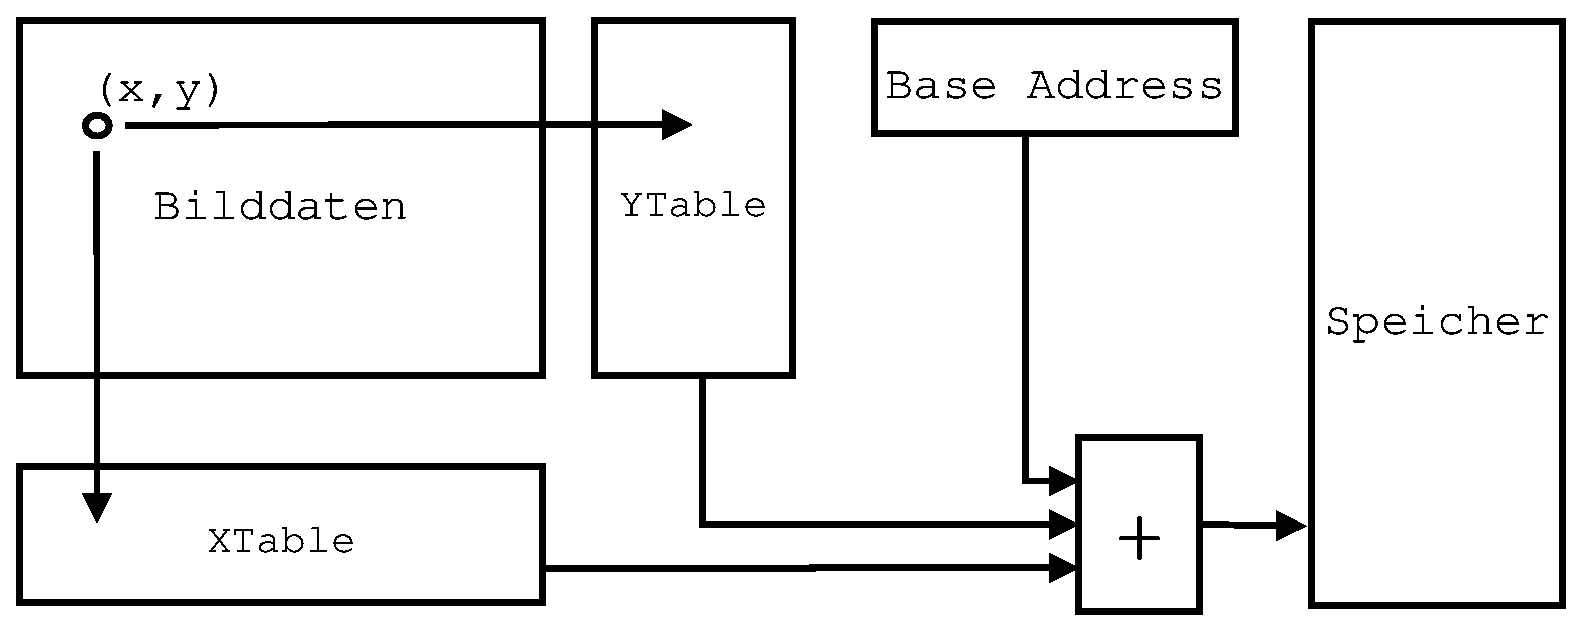
\includegraphics[width=0.9\textwidth]{images/vpa1.eps}
\caption{Pixeladressierung mit VPA} \label{pic_vpa1}
\end{center}
\end{figure}

In~\cite{zamperoni} steht dies und das\ldots

\subsection{Aufbau}

%\include{blabla} ..... usw.

%------ appendix ------
\appendix

%%%%%%%%%%%%%%%%%%%%%%%%%%%%%%%%%%%%%%%%%%%%%%%%%%%%%%%%%%%%%%%%%
% Contents: Appendix - Diplomarbeit, FH Regensburg              %
%                          11.03.2003                           %
%---------------------------------------------------------------%
%                         Anhang.tex                            %
%                      by Vorname Nachname                      %
%                         mail@mail.com                         %
%%%%%%%%%%%%%%%%%%%%%%%%%%%%%%%%%%%%%%%%%%%%%%%%%%%%%%%%%%%%%%%%%

\chapter{Dieses und jenes}


\chapter{noch was}

%%%%%%%%%%%%%%%%%%%%%%%%%%%%%%%%%%%%%%%%%%%%%%%%%%%%%%%%%%%%%%%%%
% Contents: Bibliography - Diplomarbeit, FH Regensburg          %
%                          11.03.2003                           %
%---------------------------------------------------------------%
%                         Literatur.tex                         %
%                      by Vorname Nachname                      %
%                         mail@mail.com                         %
%%%%%%%%%%%%%%%%%%%%%%%%%%%%%%%%%%%%%%%%%%%%%%%%%%%%%%%%%%%%%%%%%

\begin{thebibliography}{99}
\addcontentsline{toc}{chapter}{Literaturverzeichnis}

\bibitem{ImageNation}
  \textsc{Imagenation Corporation}:
  \textsl{User's Guide for the PX510 and PX610}.
  ImageNation Systems, September 1997

\bibitem{platt}
  \textsc{Platt, David S.}:
  \textsl{The essence of COM and ActiveX: a programmers workbook}.
  2nd~Edition, Prentice Hall, 1998

\bibitem{isernhagen}
  \textsc{Isernhagen, Rolf}:
  \textsl{Softwaretechnik in C und C++}.
  2.~Auflage, Carl-Hanser-Verlag, 2000

\bibitem{sphar}
  \textsc{Sphar, Chuck}:
  \textsl{Visual C++ 6}.
  Microsoft Press Deutschland, 1999

\bibitem{zamperoni}
  \textsc{Zamperoni, Piero}:
  \textsl{Methoden der digitalen Bildsignalverarbeitung}.
  5.~Auflage, Springer-Verlag, 2002

\bibitem{url_directx}
  \verb|http://www.microsoft.com/windows/directx|\\
  Microsoft DirectX Homepage

\bibitem{url_mfc}
  \verb|http://msdn.microsoft.com|\\
  Microsoft Developer Network - MSDN

\bibitem{url_lexikon}
  \verb|http://entwickler.com/itr/psecom,id,84,nodeid,.html|\\
  entwickler.com - Lexikon

\end{thebibliography}

%%%%%%%%%%%%%%%%%%%%%%%%%%%%%%%%%%%%%%%%%%%%%%%%%%%%%%%%%%%%%%%%%
% Contents: Erkl�rung - Diplomarbeit, FH Regensburg             %
%                          11.03.2003                           %
%---------------------------------------------------------------%
%                         Erklaerung.tex                        %
%                      by Vorname Nachname                      %
%                         mail@mail.com                         %
%%%%%%%%%%%%%%%%%%%%%%%%%%%%%%%%%%%%%%%%%%%%%%%%%%%%%%%%%%%%%%%%%

\chapter*{Erkl�rung}
\addcontentsline{toc}{chapter}{Erkl�rung}
\begin{enumerate}
\item Mir ist bekannt, dass die Diplomarbeit als Pr�fungsleistung in
  das Eigentum des Freistaats Bayern �bergeht. Hiermit erkl�re ich
  mein Einverst�ndnis, dass die Fachhochschule Regensburg diese
  Pr�fungsleistung den Studenten der Fachhochschule Regensburg
  einsehen lassen darf, und dass sie die Abschlussarbeit unter Nennung
  meines Namens als Urheber ver�ffentlichen darf.

\item Ich erkl�re hiermit, dass ich diese Diplomarbeit selbst�ndig
  verfa�t, noch nicht anderweitig f�r andere Pr�fungszwecke vorgelegt,
  keine anderen als die angegebenen Quellen und Hilfsmittel ben�tzt
  sowie w�rtliche und sinngem��e Zitate als solche gekennzeichnet
  habe.
\end{enumerate}
\vspace{4cm} Regensburg, den 11.03.2003


%------ end of document ------
\end{document}
